\subsection{Simulating Shadowing Cables as Opaque Cylinders}
\label{sec:cables}

The main cable of each detector string (figure \ref{fig:ahyoi7Ma})
allows to power the detector modules and to transfer data from the
modules to the surface. The cable has a diameter of \(46\mm\)
\cite{instrumentation} and, as it is located in close proximity to the
optical modules, shields the optical modules from a non-negligible
amount of incoming photons. The cable's mantle is black such that it
will absorb photons rather than reflect them.

\begin{figure}[htbp]
  \subcaptionbox{Optical module deployment schematics. Image source:  \cite{instrumentation}}{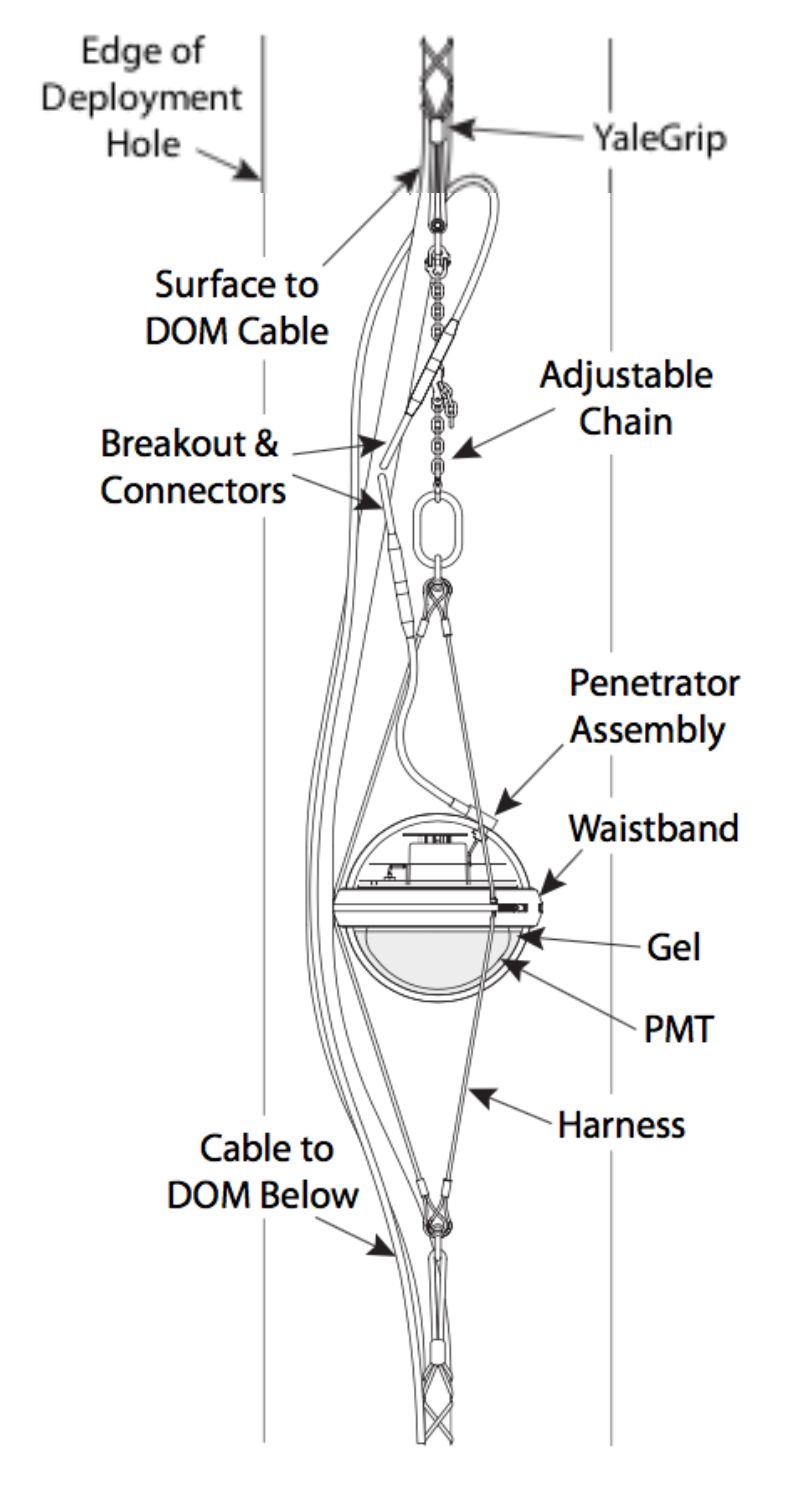
\includegraphics[width=0.25\textwidth]{img/dom-cable-instrumentation}}\hfill
  \subcaptionbox{Rendered image of the optical module and the main cable. Image source: \cite{gallerydomcloseup}}{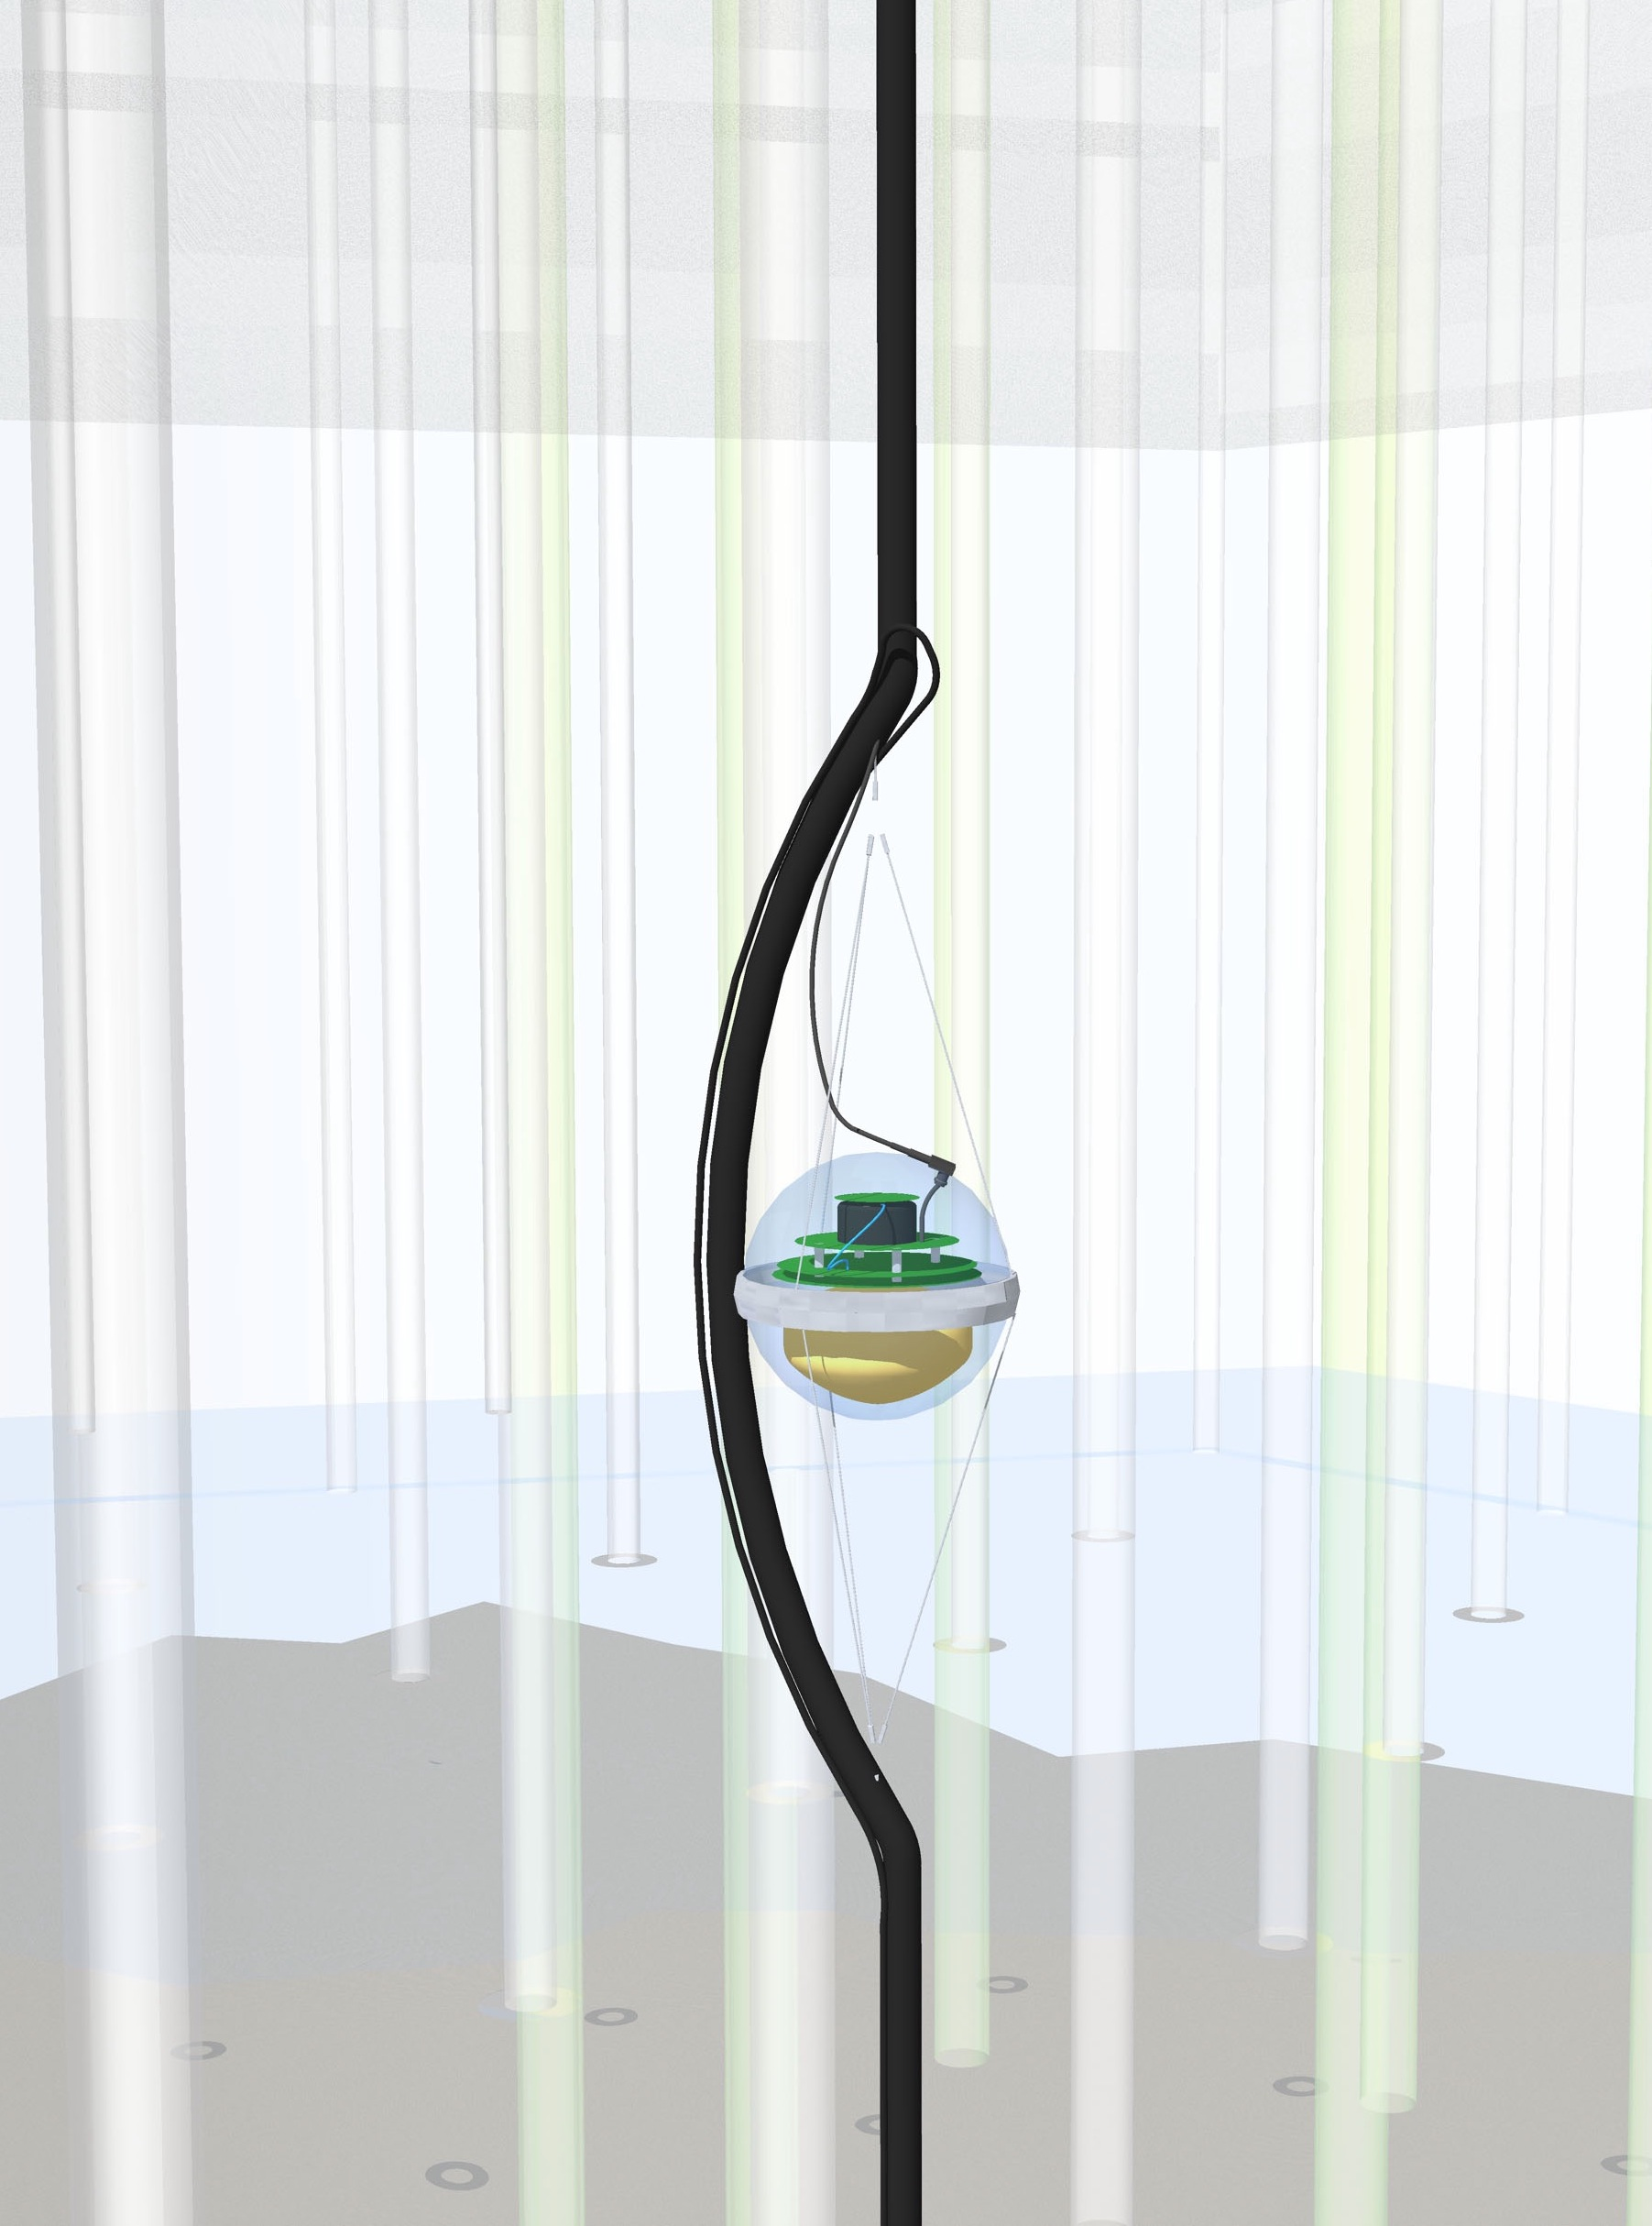
\includegraphics[width=0.35\textwidth]{img/DOMCloseUp-cropped-mirrored}}\hfill
  \subcaptionbox{Photo: Optical module deployment. Image source: \cite{publicgallerydomdeployment}}{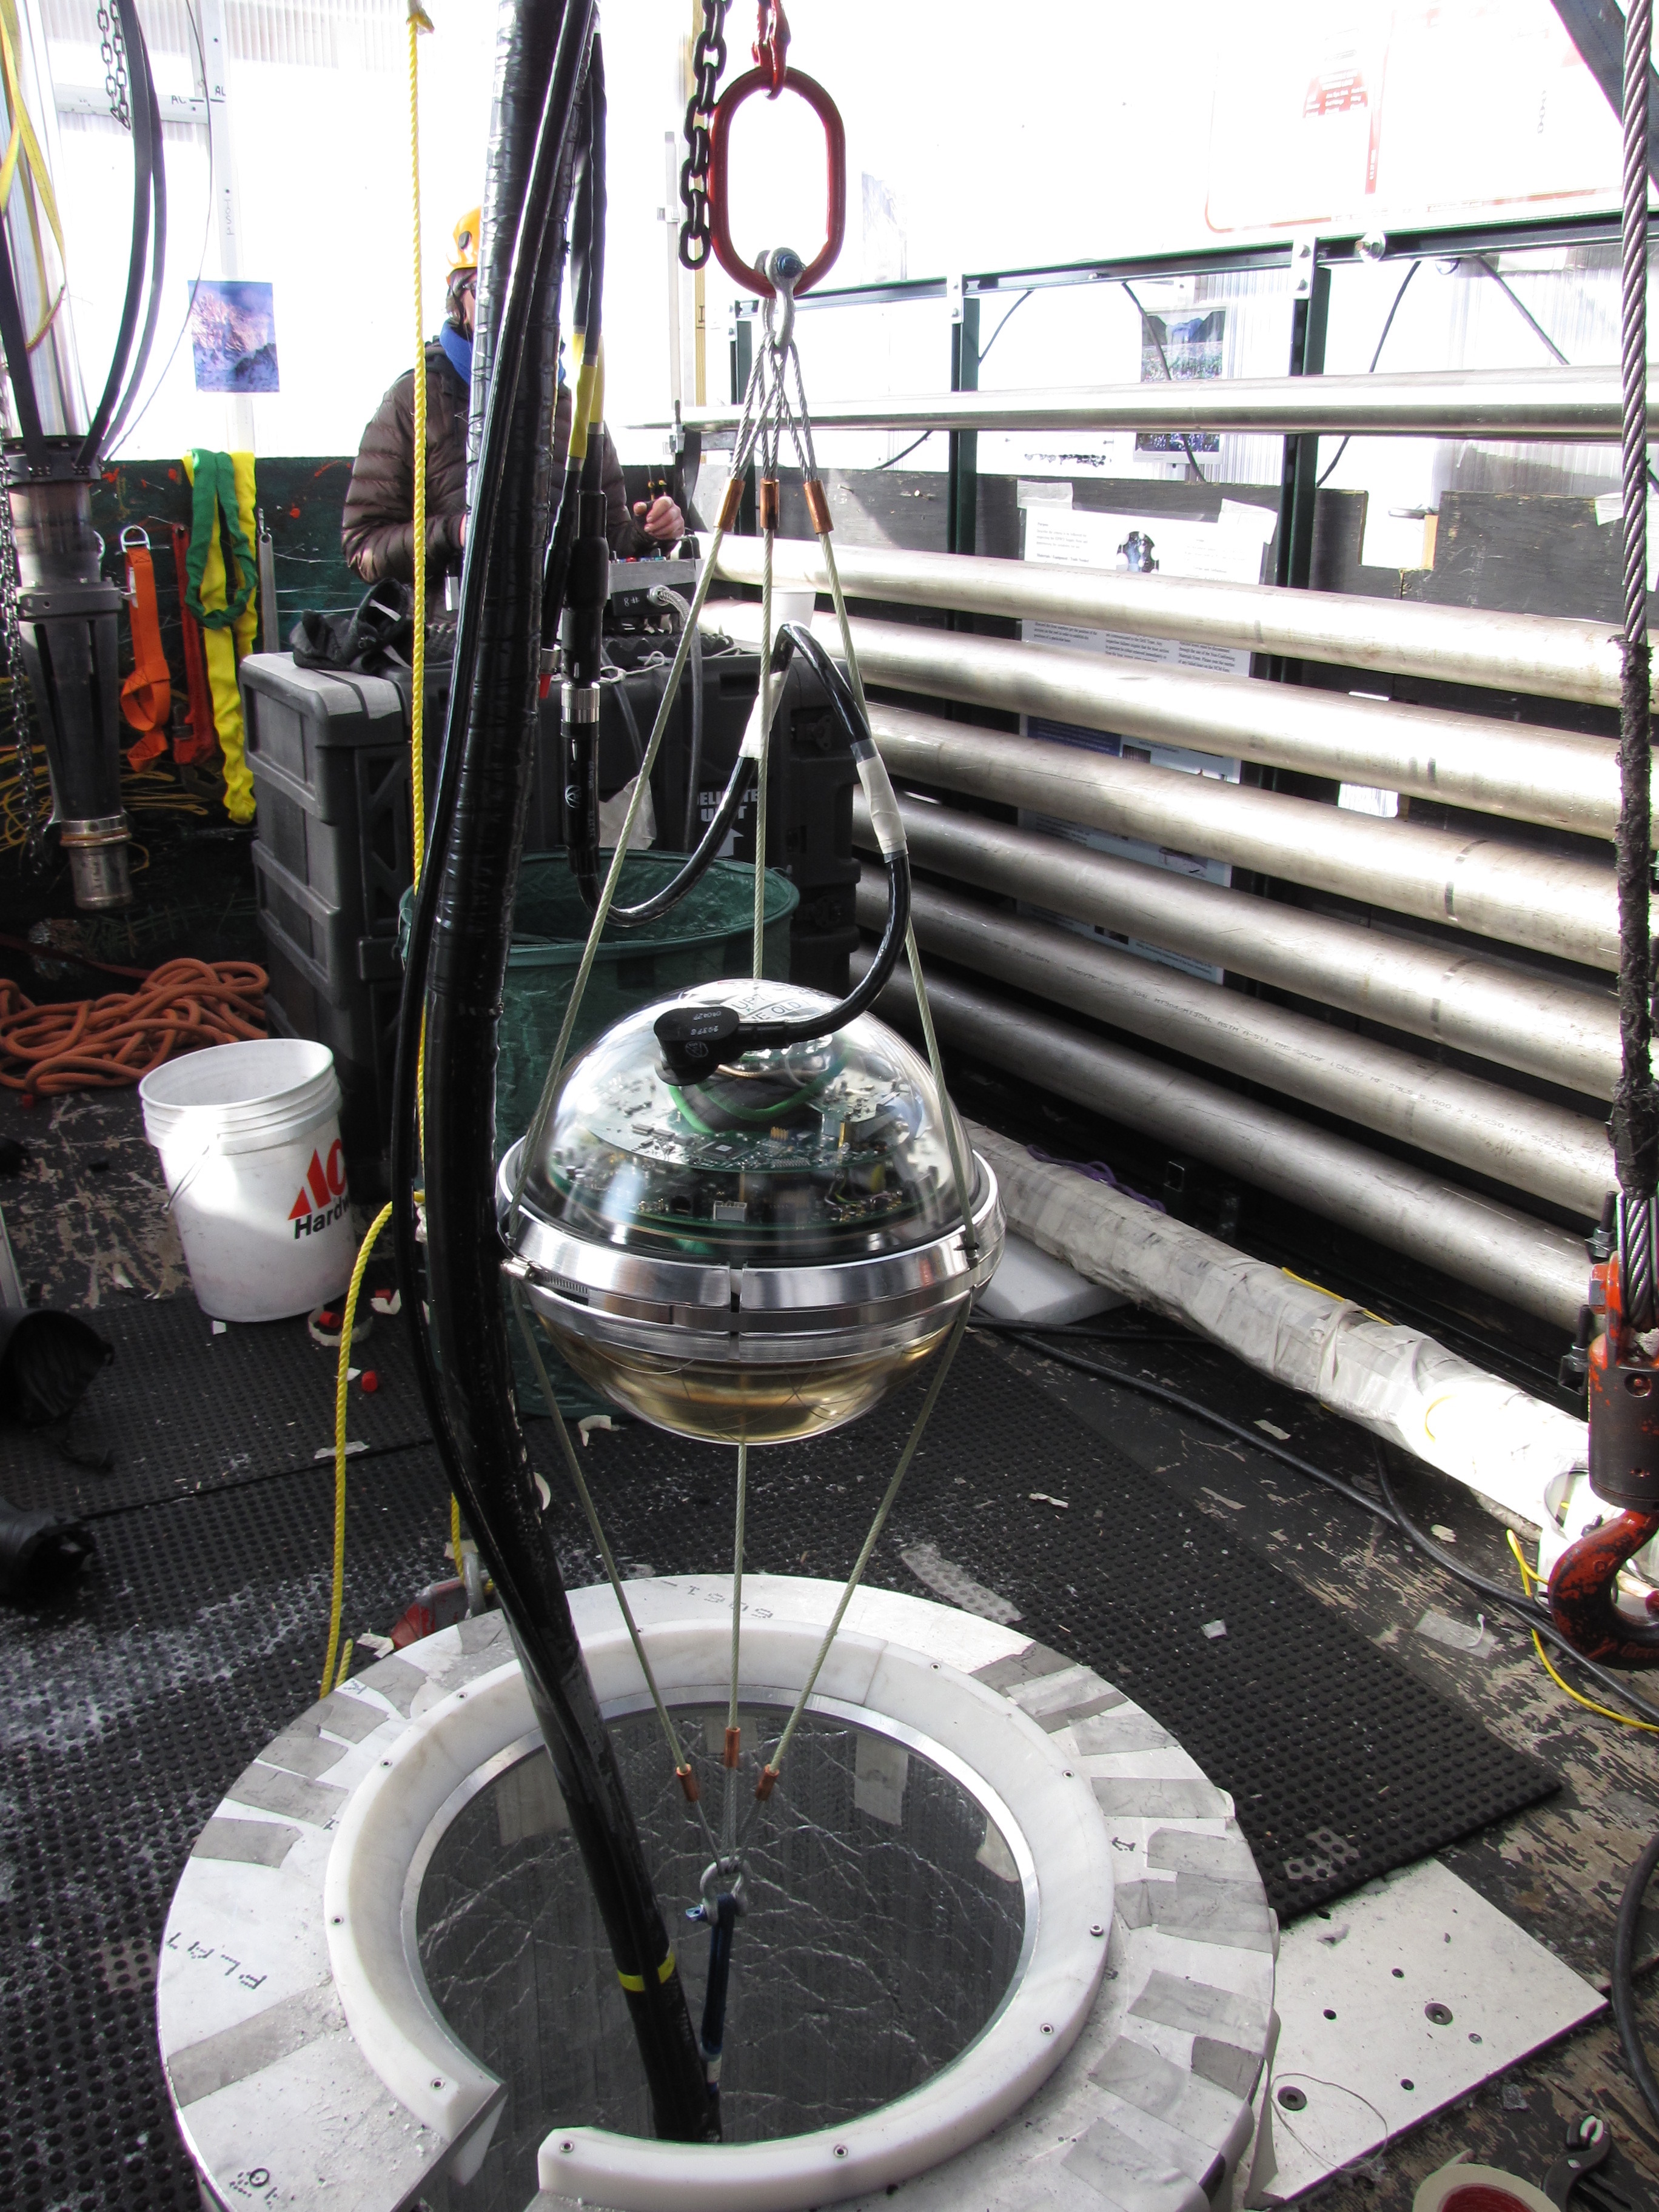
\includegraphics[width=0.35\textwidth]{img/dom-deployment-15-IMG_0080-652058109-3}}
  \caption{\icecube's optical module in relation to the main cable.}
  \label{fig:ahyoi7Ma}
\end{figure}

\subsubsection{Asymmetric Shadowing Effect Caused by the Cable}

Using the new medium-propagation algorithm, the cable can be simulated
as one or several cylinders with limited \(z\)-range, which are
configured for instant absorption.

As a first test, a simulation is performed to verify that the cable
causes an asymmetric shadowing effect, shielding photons approaching
from one direction while not shielding photons approaching from the
opposite direction. Figure \ref{fig:ochoCh7o} shows the effective
angular sensitivity of the optical module measured in this simulation
and confirms that the asymmetric shadowing can be observed in
simulations.

\docpar{This simulation, placing an opaque cylinder part besides the optical module, propagating the photons with the hole-ice-correction algorithm (section \ref{sec:algorithm_a}) and scanning the effective angular acceptance, is documented in \issue{35}.}

\begin{figure}[htbp]
  \subcaptionbox{\steamshovel visualization of the simulation scenario. Photons approaching from different angles are either shielded by the cable or can reach the optical module unhindered.}{\halfimage{cable-shadow-steamshovel-commented}\vspace*{7mm}}\hfill
  \subcaptionbox{Effective angular acceptance of the optical module measured in the simulation. Photons approaching from the side of the cable are less likely to reach the optical module and be registered as a hit.}{\halfimage{cable-shadow-angular-acceptance-commented}}
  \caption{Simulation with the main cable modeled as opaque cylinder placed besides the optical module.}
  \label{fig:ochoCh7o}
\end{figure}

\subsubsection{Cable Inside the Bubble Column}

In one class of hole-ice models that has not been studied with
simulations, yet, the optical module is shifted such that the cable
resides fully or partially within the bubble column.
\cite{martinspicehddard}

\begin{figure}[htbp]
  \subcaptionbox{\steamshovel visualization of the simulation scenario. An opaque cable cylinder of $1\m$ height is placed besides the optical module, fully within the drill hole ice, and partially inside the bubble column.}{\halfimage{cable-inside-shifted-bc-steamshovel}\vspace*{4mm}}\hfill
  \subcaptionbox{Effective angular acceptance of the optical module measured in simulations with and without cable.}{\halfimage{cable-inside-shifted-bc-angular-acceptance}}\hfill
  \caption{Simulation with opaque cable partially inside bubble column.}
  \label{fig:caweNg6o}
\end{figure}

Placing a minimal opaque cable cylinder besides the optical module
partially inside the bubble column in a simulation, using plane waves as
photon sources, direct detection as hit acceptance criterion, and the
new medium-propagation algorithm (section \ref{sec:algorithm_b}), the
cable shadowing effect appears to be subdominant when measuring the
effective angular acceptance (figure \ref{fig:caweNg6o}) compared to the
effect of the bubble column and the drill hole ice. For photons
approaching the optical module from the side where the cable is located,
the number of photon hits is decreased compared to a simulation without
cable. But the effect is smaller than the statistical error.

\docpar{This simulation is documented in \issue{110}.}

\subsubsection{Can Cable Effects Account for the Observed Hole-Ice Effects?}

An open question raised by the \icecube Calibration Group is whether the
shielding by the main cable is sufficient to account for the effects
observed by other studies that are typically attributed to the hole
ice.\footnote{Internal correspondence. See for example \url{https://icecube-spno.slack.com/archives/C4FV72473/p1522086838000178}.}

The following series of simulations compares the effective angular
acceptance for a scenario where only a shadowing cable is considered,
and a typical drill-hole-ice scenario. This simulation uses the new
medium-propagation algorithm (section \ref{sec:algorithm_b}), plane
waves as photon sources, and direct detection as hit acceptance
criterion. The cable is modeled as three opaque cylinder parts (see
figure \ref{fig:Ohw1aibu} (a) in comparison to the illustrations in
figure \ref{fig:ahyoi7Ma}). The drill-hole ice is modeled with
properties suggested by the so-called \textit{H2 model}, a
hole-ice-cylinder radius of \(30\cm\) and a geometric scattering length
of \(50\cm\) \cite{holeicestudieswithyag}.

\docpar{This series of simulations is documented in \issue{101}.}

\begin{figure}[htbp]
  \subcaptionbox{\steamshovel visualization of the simulation scenario with cables: The cable is modeled as three opaque cylinder parts. See also figure \ref{fig:ahyoi7Ma} for comparison.}{\halfimage{cable-only-vs-h2-steamshovel}\vspace*{3mm}}\hfill
  \subcaptionbox{Effective angular acceptance curves for the optical module measured in simulations without hole ice, with only a cable, and with a hole-ice-cylinder of $30\cm$ radius and a geometric hole-ice scattering length of $50\cm$ (H2 model parameters).}{\halfimage{cable-only-vs-h2-angular-acceptance}}\hfill
  \caption{Measuring the effective angular acceptance of an optical module in simulations: (1) without hole ice, (2) with only a drill hole, (3) with only a cable.}
  \label{fig:Ohw1aibu}
\end{figure}

As shown in figure \ref{fig:Ohw1aibu} (b), the cable can account for a
total reduction in photon hits. For the decreased number of hits for
photons approaching from below, and an increased number of hits for
photons approaching from above, however, which are expected from earlier
hole-ice studies (see section \ref{sec:hole_ice_approximation}), the
simulated cable cannot account for.
